\documentclass[9pt,aspectratio=169]{beamer}
\usetheme{StAndrews}

\coursename{FI5699 Dissertation Module}
\graphicspath{ {./logos/} {./outputs/} {./pix/week4/} }
\title{\LARGE \textnormal{Week 4: \\
Working with Data in Python}}
\hypersetup{pdftitle={FI5699 Week 4 -- Working with Data in Python}}

% ============================================================================
% CODE LISTINGS SETUP
% ============================================================================
\usepackage{listings}
\lstset{
  language=Python,
  basicstyle=\ttfamily\footnotesize,
  keywordstyle=\color{StAndrewsBlue}\bfseries,
  stringstyle=\color{StAndrewsMidGreen},
  commentstyle=\color{StAndrewsOrange}\itshape,
  numberstyle=\tiny\color{gray},
  numbers=left,
  numbersep=5pt,
  backgroundcolor=\color{gray!5},
  frame=single,
  rulecolor=\color{StAndrewsBlue!30},
  breaklines=true,
  showstringspaces=false,
  tabsize=4,
  xleftmargin=1.5em,
  framexleftmargin=1em,
  captionpos=b,
  morekeywords={True, False, None, print, range, len, sum, max, min, type,
                exit, int, float, str, bool, import, as, from, for, in,
                while, def, return, class, with, open, f},
  literate={>>>}{{\textcolor{StAndrewsBurgundy}{>{>}>}}}3,
}

% Inline code command
\newcommand{\py}[1]{\lstinline[language=Python]{#1}}

% Shell listing style (for terminal commands)
\lstdefinestyle{shell}{
  language={},
  basicstyle=\ttfamily\footnotesize,
  keywordstyle={},
  stringstyle={},
  commentstyle=\color{StAndrewsOrange}\itshape,
  backgroundcolor=\color{gray!5},
  frame=single,
  rulecolor=\color{StAndrewsBlue!30},
  numbers=none,
  xleftmargin=1.5em,
  framexleftmargin=1em,
  breaklines=true,
  showstringspaces=false,
  literate={~}{{\raise.25ex\hbox{$\sim$}}}1
           {\$}{{\textcolor{StAndrewsMidGreen}{\$}}}1,
}

% Output style (for Python output, light blue border)
\lstdefinestyle{output}{
  language={},
  basicstyle=\ttfamily\scriptsize,
  keywordstyle={},
  stringstyle={},
  commentstyle={},
  backgroundcolor=\color{gray!3},
  frame=single,
  rulecolor=\color{StAndrewsLightBlue!50},
  numbers=none,
  xleftmargin=0.5em,
  framexleftmargin=0.2em,
  breaklines=true,
  showstringspaces=false,
}

% ============================================================================
% ADDITIONAL PACKAGES
% ============================================================================
\usepackage{tcolorbox}

% Custom table column types
\newcolumntype{R}{>{\raggedright\arraybackslash}p{8cm}}

% Highlight box (encouragement / key takeaways)
\newtcolorbox{highlightbox}{
  colback=StAndrewsLightBlue!8,
  colframe=StAndrewsBlue!25,
  boxrule=0.8pt,
  arc=4pt,
  left=6pt, right=6pt,
  top=4pt, bottom=4pt,
}

% Demo box (live demonstration callouts)
\newtcolorbox{demobox}[1][Live Demonstration]{
  colback=StAndrewsBlue!5,
  colframe=StAndrewsBlue!50,
  boxrule=0.8pt,
  arc=4pt,
  left=6pt, right=6pt,
  top=4pt, bottom=4pt,
  fonttitle=\bfseries,
  title=#1,
}


\begin{document}

% ============================================================================
% TITLE PAGE
% ============================================================================
\begin{frame}[plain]
\titlepage
\end{frame}


% ============================================================================
% SECTION 0: OPENING
% ============================================================================
\section{Introduction}
\subsection{Roadmap}

\begin{frame}{What We Will Cover Today}

This is a \alert{hands-on session}. You are welcome to have your laptop open and follow along.

\medskip

\begin{enumerate}
    \item \textbf{Polars Data Structures} --- DataFrames, Series, and data types
    \item \textbf{Reading \& Writing Data} --- CSV and Excel I/O with Polars
    \item \textbf{Expressions \& Contexts} --- the Polars way of querying data
    \item \textbf{Working with Expressions} --- arithmetic, comparisons, conditionals
    \item \textbf{Working with Stock Returns} --- downloading Yahoo Finance data
    \item \textbf{Combining DataFrames} --- joins and concatenation
    \item \textbf{Reshaping Data} --- pivot and unpivot
    \item \textbf{Visualising Data} --- building plots with \texttt{plotnine}
\end{enumerate}

\medskip

\begin{highlightbox}
\centering
By the end of today, you will be able to load real financial data, query, transform, reshape, and visualise it in Python.
\end{highlightbox}

\end{frame}


\begin{frame}{Table of Contents}
\footnotesize
\begin{columns}[t]
  \begin{column}{0.33\textwidth}
    \tableofcontents[sections={1-4}]
  \end{column}
  \begin{column}{0.33\textwidth}
    \tableofcontents[sections={5-7}]
  \end{column}
  \begin{column}{0.33\textwidth}
    \tableofcontents[sections={8-10}]
  \end{column}
\end{columns}
\end{frame}


\subsection{Recap}
\begin{frame}{Recap: What You Built in Week 2}

\begin{tabular}{@{}lp{8cm}@{}}
\toprule
\textbf{Concept} & \textbf{What you learned} \\
\midrule
Positron & Console, Terminal, and Editor \\[0.3em]
\texttt{uv} & \texttt{uv init}, \texttt{uv add} to manage packages \\[0.3em]
Variables & \py{price = 142.50}, types (\py{int}, \py{float}, \py{str}, \py{bool}) \\[0.3em]
Lists \& Dicts & \texttt{["AAPL", "MSFT"]} and \texttt{\{"ticker": "AAPL"\}} \\[0.3em]
Loops & \py{for} and \py{while} --- automating repetitive tasks \\
\bottomrule
\end{tabular}

\bigskip

\begin{highlightbox}
\centering
Today we move from Python basics to \textbf{working with real data} using \texttt{polars} and \texttt{plotnine}.
\end{highlightbox}

\end{frame}


\subsection{Getting Started}

\begin{frame}[fragile]{Companion Code: \texttt{week-4-code}}

Every concept in this lecture has a runnable Python script in the \texttt{week-4-code} folder.

\medskip

\begin{tabular}{@{}ll@{}}
\toprule
\textbf{Script} & \textbf{Covers} \\
\midrule
\texttt{01\_data\_structures.py}        & DataFrames, Series, types, nulls \\[0.2em]
\texttt{02\_reading\_writing\_data.py}  & CSV \& Excel I/O \\[0.2em]
\texttt{03\_expressions\_contexts.py}   & select, with\_columns, filter, group\_by \\[0.2em]
\texttt{04\_working\_with\_expressions.py} & Arithmetic, conditionals, casting \\[0.2em]
\texttt{05\_real\_stock\_data.py}       & Yahoo Finance data \& returns \\[0.2em]
\texttt{06\_combining\_dataframes.py}   & Joins \& concatenation \\[0.2em]
\texttt{07\_reshaping\_data.py}         & Pivot \& unpivot \\[0.2em]
\texttt{08\_visualising\_data.py}       & plotnine charts \\
\bottomrule
\end{tabular}

\medskip

\begin{highlightbox}
\centering
Open \texttt{week-4-code} in Positron and run each script to see the concepts in the .py files.
\end{highlightbox}

\end{frame}


\begin{frame}[fragile]{Setting Up: Two Steps}

\begin{enumerate}
    \item \textbf{Open the folder in Positron}

    \smallskip

    \texttt{File} $\to$ \texttt{Open Folder\ldots} $\to$ select \texttt{week-4-code}

    \bigskip

    \item \textbf{Install dependencies}

    \smallskip

    Open a Terminal in Positron and run:

\begin{lstlisting}[basicstyle=\ttfamily\small]
uv sync
\end{lstlisting}

    This reads \texttt{pyproject.toml} and installs Polars, plotnine, tidyfinance, and all other packages into a virtual environment.

    \bigskip

    \item \textbf{Select the interpreter}

    \smallskip

    Click \texttt{Select Interpreter} in the top-right corner of Positron and choose the \texttt{.venv} Python that \texttt{uv sync} just created. This ensures Positron uses the correct packages when you run scripts.
\end{enumerate}

\bigskip

\begin{highlightbox}
\centering
Once the interpreter is set, you are ready to go.\\
Open any script and press \texttt{Ctrl+Shift+Enter} to run it.
\end{highlightbox}

\end{frame}


\subsection{Motivation}
\begin{frame}{From Lists to DataFrames}

In Week 2 you used lists and dictionaries to organise small amounts of data. But your dissertation will involve \alert{thousands of rows} --- stock prices, returns, firm characteristics.

\medskip

\begin{tabular}{@{}llp{5.5cm}@{}}
\toprule
 & \textbf{Lists / Dicts} & \textbf{Polars} \\
\midrule
\textbf{Data size} & A handful of values & Millions of rows \\[0.3em]
\textbf{Operations} & One value at a time & Entire columns at once \\[0.3em]
\textbf{Speed} & Pure Python (slow) & Written in Rust (fast) \\[0.3em]
\textbf{Structure} & Ad hoc & Typed columns, schemas \\
\bottomrule
\end{tabular}

\bigskip

Think of Polars as a \textbf{supercharged spreadsheet} that you control with code.

\end{frame}


% ============================================================================
% SECTION 1: POLARS DATA STRUCTURES
% ============================================================================
\section{Polars Data Structures}
\subsection{The DataFrame}

\begin{frame}{A DataFrame Is a Table with Typed Columns}

\begin{columns}[T]
\begin{column}{0.55\textwidth}
A \alert{DataFrame} is the core Polars data structure:

\medskip

\bi
    \item A table of rows and columns --- like a spreadsheet
    \item Each column has a \textbf{name} and a \textbf{data type}
    \item Each column is internally a \alert{Series}
    \item All values in a column share the same type
    \item Different columns can have different types
\ei
\end{column}
\begin{column}{0.42\textwidth}
\centering
\begin{tikzpicture}[
  cell/.style={rectangle, minimum width=1.6cm, minimum height=0.5cm,
               draw=StAndrewsBlue!30, font=\tiny, anchor=center},
  header/.style={cell, fill=StAndrewsBlue, text=white, font=\tiny\bfseries},
  type/.style={cell, fill=StAndrewsBlue!10, font=\tiny\itshape},
]
  % Headers
  \node[header] (h1) at (0,0) {ticker};
  \node[header] (h2) at (1.7,0) {price};
  \node[header] (h3) at (3.4,0) {shares};

  % Types
  \node[type] (t1) at (0,-0.5) {str};
  \node[type] (t2) at (1.7,-0.5) {f64};
  \node[type] (t3) at (3.4,-0.5) {i64};

  % Data rows
  \node[cell] at (0,-1.0) {AAPL};
  \node[cell] at (1.7,-1.0) {189.84};
  \node[cell] at (3.4,-1.0) {50};

  \node[cell] at (0,-1.5) {MSFT};
  \node[cell] at (1.7,-1.5) {378.91};
  \node[cell] at (3.4,-1.5) {30};

  \node[cell] at (0,-2.0) {TSLA};
  \node[cell] at (1.7,-2.0) {248.42};
  \node[cell] at (3.4,-2.0) {20};

  % Labels
  \draw[<-, StAndrewsBlue, thick] (3.4,-1.0) -- ++(1.0,0)
    node[right, font=\tiny] {Row};
  \draw[<-, StAndrewsBlue, thick] (1.7,0.0) -- ++(0,0.5)
    node[above, font=\tiny] {Column (Series)};
\end{tikzpicture}
\end{column}
\end{columns}

\end{frame}


\begin{frame}[fragile]{Creating Your First Polars DataFrame}

\begin{lstlisting}
import polars as pl

stocks = pl.DataFrame({
    "ticker": ["AAPL", "MSFT", "TSLA", "AMZN", "GOOGL"],
    "price":  [189.84, 378.91, 248.42, 178.25, 141.80],
    "shares": [50, 30, 20, 40, 35],
    "sector": ["Tech", "Tech", "Auto", "Retail", "Tech"],
})
print(stocks)
\end{lstlisting}

\begin{lstlisting}[style=output]
shape: (5, 4)
+--------+--------+--------+--------+
| ticker | price  | shares | sector |
| ---    | ---    | ---    | ---    |
| str    | f64    | i64    | str    |
+========+========+========+========+
| AAPL   | 189.84 | 50     | Tech   |
| MSFT   | 378.91 | 30     | Tech   |
| TSLA   | 248.42 | 20     | Auto   |
| AMZN   | 178.25 | 40     | Retail |
| GOOGL  | 141.8  | 35     | Tech   |
+--------+--------+--------+--------+
\end{lstlisting}

\end{frame}


\subsection{Data Types}
\begin{frame}{Every Column Has a Data Type}

Polars \alert{infers} types automatically, but it helps to know the common ones:

\medskip

\begin{tabular}{@{}llp{5cm}@{}}
\toprule
\textbf{Type} & \textbf{Polars name} & \textbf{Example values} \\
\midrule
Whole number & \texttt{Int64} & Shares: 50, 30, 20 \\[0.3em]
Decimal number & \texttt{Float64} & Price: 189.84, 378.91 \\[0.3em]
Text & \texttt{String} & Ticker: ``AAPL'', ``MSFT'' \\[0.3em]
True / False & \texttt{Boolean} & Is profitable: true, false \\[0.3em]
Date & \texttt{Date} & 2024-01-15 \\[0.3em]
Date + time & \texttt{Datetime} & 2024-01-15 09:30:00 \\[0.3em]
Missing value & \texttt{Null} & Unknown or not applicable \\
\bottomrule
\end{tabular}

\medskip

\begin{highlightbox}
\centering
You can see each column's type in the \texttt{---} row of the printed output.
\end{highlightbox}

\end{frame}


\begin{frame}[fragile]{A Series Is a Single Column}

A \alert{Series} is a one-dimensional array --- one column of a DataFrame:

\begin{lstlisting}
prices = pl.Series("price", [189.84, 378.91, 248.42])
print(prices)
print(f"Type:  {prices.dtype}")
print(f"Mean:  {prices.mean():.2f}")
\end{lstlisting}

\begin{lstlisting}[style=output]
shape: (3,)
Series: 'price' [f64]
[
    189.84
    378.91
    248.42
]
Type:  Float64
Mean:  272.39
\end{lstlisting}

You rarely create Series directly --- they arise when you extract a column from a DataFrame.

\end{frame}


\subsection{Inspecting Data}
\begin{frame}[fragile]{Five Ways to Look at Your Data}

\begin{tabular}{@{}lp{5cm}l@{}}
\toprule
\textbf{Method} & \textbf{What it shows} & \textbf{Example} \\
\midrule
\py{.head(n)} & First \texttt{n} rows (default 5) & \py{stocks.head(3)} \\[0.5em]
\py{.tail(n)} & Last \texttt{n} rows & \py{stocks.tail(3)} \\[0.5em]
\py{.shape} & (rows, columns) tuple & \py{stocks.shape} \\[0.5em]
\py{.columns} & List of column names & \py{stocks.columns} \\[0.5em]
\py{.schema} & Column names and types & \py{stocks.schema} \\
\bottomrule
\end{tabular}

\bigskip

\begin{lstlisting}
print(stocks.shape)
print(stocks.columns)
\end{lstlisting}

\begin{lstlisting}[style=output]
(5, 4)
['ticker', 'price', 'shares', 'sector']
\end{lstlisting}

\end{frame}


\begin{frame}[fragile]{Summary Statistics with \texttt{describe()}}

\begin{lstlisting}
print(stocks.describe())
\end{lstlisting}

\begin{lstlisting}[style=output]
shape: (9, 5)
+------------+--------+-----------+----------+--------+
| statistic  | ticker | price     | shares   | sector |
| ---        | ---    | ---       | ---      | ---    |
| str        | str    | f64       | f64      | str    |
+============+========+===========+==========+========+
| count      | 5      | 5.0       | 5.0      | 5      |
| null_count | 0      | 0.0       | 0.0      | 0      |
| mean       | null   | 227.444   | 35.0     | null   |
| std        | null   | 92.939425 | 11.18034 | null   |
| min        | AAPL   | 141.8     | 20.0     | Auto   |
| 25%        | null   | 178.25    | 30.0     | null   |
| 50%        | null   | 189.84    | 35.0     | null   |
| 75%        | null   | 248.42    | 40.0     | null   |
| max        | TSLA   | 378.91    | 50.0     | Tech   |
+------------+--------+-----------+----------+--------+
\end{lstlisting}

One command gives you count, mean, standard deviation, min, max, and quartiles --- the same summary statistics you would compute in Excel or Stata.

\end{frame}


\begin{frame}[fragile]{Null Means Missing}

Polars uses \py{null} for missing data. Every data type supports it --- unlike Excel's blank cells, a \py{null} is explicit and typed.

\bigskip

\begin{columns}[T]
\begin{column}{0.48\textwidth}
\textbf{Why it matters:}
\bi
    \item Real-world data has gaps (no price on a holiday, missing filings)
    \item Polars propagates \py{null} through calculations: \texttt{null + 5 = null}
    \item You can detect them with \py{.is_null()} or fill them with \py{.fill_null()}
\ei
\end{column}
\begin{column}{0.48\textwidth}
\textbf{\texttt{null} vs \texttt{NaN}:}
\bi
    \item \texttt{null} = ``no value exists''
    \item \texttt{NaN} = ``a float calculation failed'' (e.g.\ 0/0)
    \item In Polars, use \py{null} for missing data
    \item \texttt{NaN} is only for \texttt{Float64} columns
\ei
\end{column}
\end{columns}

\bigskip

\begin{highlightbox}
\centering
When you see \texttt{null} in your output, it means the data is \textbf{genuinely missing}, not zero.
\end{highlightbox}

\end{frame}


\subsection{Exercises}
\begin{frame}[fragile]{Exercise 1: Build and Inspect a DataFrame}

\begin{alertblock}{Try It Yourself (5 minutes)}
\begin{enumerate}
    \item Create a new file \texttt{week4.py} and add \py{import polars as pl} at the top
    \item Create a DataFrame called \texttt{portfolio} with columns:
    \begin{itemize}
        \item \texttt{"ticker"}: at least 4 stocks you know
        \item \texttt{"price"}: a price for each (make them up)
        \item \texttt{"shares"}: how many shares of each
    \end{itemize}
    \item Print the DataFrame
    \item Print \py{portfolio.shape} and \py{portfolio.describe()}
    \item \textbf{Bonus:} Create a \py{pl.Series} of monthly returns and compute its \py{.mean()}
\end{enumerate}
\end{alertblock}

\end{frame}


% ============================================================================
% SECTION 2: READING AND WRITING DATA
% ============================================================================
\section{Reading and Writing Data}
\subsection{CSV Files}

\begin{frame}[fragile]{Reading a CSV File}

Most financial data starts life as a CSV file. Polars reads them with \py{pl.read_csv()}:

\begin{lstlisting}
import polars as pl

df = pl.read_csv("stock_prices.csv")
print(df.head())
\end{lstlisting}

\medskip

\begin{tabular}{@{}lp{7.5cm}@{}}
\toprule
\textbf{Function} & \textbf{What it does} \\
\midrule
\py{pl.read_csv(path)} & Read an entire CSV into a DataFrame immediately \\[0.3em]
\py{pl.scan_csv(path)} & Return a \texttt{LazyFrame} --- delays reading until you call \py{.collect()} \\
\bottomrule
\end{tabular}

\bigskip

\begin{highlightbox}
\centering
\texttt{scan\_csv} is faster for large files because Polars can optimise the query before reading the data.
\end{highlightbox}

\end{frame}


\begin{frame}[fragile]{Useful \texttt{read\_csv} Parameters}

\begin{lstlisting}
df = pl.read_csv(
    "stock_prices.csv",
    separator=",",          # default; use "\t" for TSV
    has_header=True,        # first row is column names
    skip_rows=0,            # skip N rows at the top
    n_rows=1000,            # read only the first 1000 rows
    null_values=["NA", ""], # treat these strings as null
    try_parse_dates=True,   # auto-detect date columns
)
\end{lstlisting}

\medskip

\begin{highlightbox}
\centering
\texttt{try\_parse\_dates=True} is especially useful for financial data --- it converts date strings into proper \texttt{Date} columns automatically.
\end{highlightbox}

\end{frame}


\begin{frame}[fragile]{Writing a CSV File}

After transforming your data, save it with \py{.write_csv()}:

\begin{lstlisting}
stocks = pl.DataFrame({
    "ticker": ["AAPL", "MSFT", "TSLA"],
    "price":  [189.84, 378.91, 248.42],
    "shares": [50, 30, 20],
})

stocks.write_csv("my_portfolio.csv")
\end{lstlisting}

\medskip

This writes a standard comma-separated file with a header row. You can customise:

\medskip

\begin{tabular}{@{}lp{6cm}@{}}
\toprule
\textbf{Parameter} & \textbf{Effect} \\
\midrule
\py{separator="\\t"} & Write a tab-separated file instead \\[0.3em]
\py{include_header=False} & Omit the header row \\
\bottomrule
\end{tabular}

\end{frame}


\begin{frame}[fragile]{Lazy Reading with \texttt{scan\_csv}}

For large files, \py{pl.scan_csv()} returns a \alert{LazyFrame} instead of loading everything:

\begin{lstlisting}
lf = pl.scan_csv("large_dataset.csv")

# Build a query without reading data yet
result = (
    lf
    .filter(pl.col("ticker") == "AAPL")
    .select("date", "close")
    .collect()  # NOW it reads and executes
)
\end{lstlisting}

\medskip

\begin{columns}[T]
\begin{column}{0.47\textwidth}
\textbf{\texttt{read\_csv}}
\bi
    \item Reads entire file immediately
    \item Returns a \texttt{DataFrame}
    \item Simple and direct
    \item Fine for small--medium files
\ei
\end{column}
\begin{column}{0.47\textwidth}
\textbf{\texttt{scan\_csv}}
\bi
    \item Defers reading until \py{.collect()}
    \item Returns a \texttt{LazyFrame}
    \item Polars optimises the query first
    \item Better for large files
\ei
\end{column}
\end{columns}

\end{frame}


\subsection{Excel Files}

\begin{frame}[fragile]{Reading Excel Files}

Polars can also read \texttt{.xlsx} files directly:

\begin{lstlisting}
df = pl.read_excel("portfolio.xlsx")

# Read a specific sheet
df = pl.read_excel("portfolio.xlsx", sheet_name="Returns")
\end{lstlisting}

\medskip

\textbf{Required dependency:} install one of these Excel engines:

\begin{lstlisting}[style=shell]
$ uv add fastexcel    # fastest (recommended, default)
$ uv add openpyxl     # slower but handles tricky files
\end{lstlisting}

\medskip

\begin{highlightbox}
\centering
Without a \texttt{sheet\_name}, Polars reads the \textbf{first sheet} by default.
\end{highlightbox}

\end{frame}


\begin{frame}[fragile]{Writing Excel Files}

Save a DataFrame to Excel with \py{.write_excel()}:

\begin{lstlisting}
stocks.write_excel("my_portfolio.xlsx")

# Specify a worksheet name
stocks.write_excel("my_portfolio.xlsx", worksheet="Holdings")
\end{lstlisting}

\medskip

\textbf{Required dependency:}
\begin{lstlisting}[style=shell]
$ uv add xlsxwriter
\end{lstlisting}

\bigskip

\begin{highlightbox}
\centering
\textbf{Performance tip:} CSV and Parquet are much faster than Excel for large datasets. Use Excel when you need to share with non-programmers; use CSV or Parquet for your own analysis pipelines.
\end{highlightbox}

\end{frame}


\subsection{Exercises}
\begin{frame}[fragile]{Exercise 2: Reading and Writing Files}

\begin{alertblock}{Try It Yourself (5 minutes)}
\begin{enumerate}
    \item Create a DataFrame with at least 4 rows of stock data (ticker, price, shares)
    \item Write it to a CSV file with \py{.write_csv("portfolio.csv")}
    \item Read it back with \py{pl.read_csv("portfolio.csv")} and print the result --- does it match?
    \item \textbf{Bonus:} Write to Excel with \py{.write_excel("portfolio.xlsx")} and read it back
    \item \textbf{Bonus:} Try \py{pl.scan_csv("portfolio.csv").collect()} --- same result?
\end{enumerate}
\end{alertblock}

\end{frame}


% ============================================================================
% SECTION 3: EXPRESSIONS AND CONTEXTS
% ============================================================================
\section{Expressions and Contexts}
\subsection{The Core Idea}

\begin{frame}{Polars Separates \emph{What} to Compute from \emph{Where}}

\begin{columns}[T]
\begin{column}{0.50\textwidth}
An \alert{expression} is a recipe for a computation. It describes \textbf{what} to do, but does nothing until you place it in a \alert{context}.

\medskip

\bi
    \item Expression: ``multiply price by shares''
    \item Context: ``add it as a new column'' or ``replace all columns'' or ``use it to filter rows''
\ei

\medskip

This separation is what makes Polars fast and flexible.
\end{column}
\begin{column}{0.47\textwidth}
\centering
\begin{tikzpicture}[node distance=0.9cm, >=stealth, thick,
  box/.style={rectangle, rounded corners=3pt, minimum width=3.2cm,
              minimum height=0.7cm, align=center, font=\scriptsize}]
  \node[box, draw=StAndrewsBlue!40, fill=StAndrewsBlue!8] (expr)
    {Expression\\[-1pt]\texttt{pl.col("price") * pl.col("shares")}};
  \node[box, below=of expr, fill=StAndrewsBlue, text=white] (ctx)
    {Context\\[-1pt]\texttt{df.select(...)}, \texttt{df.filter(...)}, \ldots};
  \node[box, below=of ctx, draw=StAndrewsBlue!40, fill=StAndrewsBlue!8] (result)
    {Result\\[-1pt]A new or modified DataFrame};
  \draw[->, StAndrewsBlue, line width=0.8pt] (expr) -- (ctx)
    node[midway, right, font=\tiny] {what};
  \draw[->, StAndrewsBlue, line width=0.8pt] (ctx) -- (result)
    node[midway, right, font=\tiny] {where};
\end{tikzpicture}
\end{column}
\end{columns}

\end{frame}


\subsection{The Four Contexts}
\begin{frame}[fragile]{Context 1: \texttt{select} --- Pick and Transform Columns}

\py{select} returns \textbf{only} the columns you ask for:

\begin{lstlisting}
result = stocks.select(
    "ticker",
    (pl.col("price") * pl.col("shares")).alias("position_value"),
)
print(result)
\end{lstlisting}

\begin{lstlisting}[style=output]
shape: (5, 2)
+--------+----------------+
| ticker | position_value |
| ---    | ---            |
| str    | f64            |
+========+================+
| AAPL   | 9492.0         |
| MSFT   | 11367.3        |
| TSLA   | 4968.4         |
| AMZN   | 7130.0         |
| GOOGL  | 4963.0         |
+--------+----------------+
\end{lstlisting}

\end{frame}


\begin{frame}[fragile]{Context 2: \texttt{with\_columns} --- Add New Columns}

\py{with_columns} keeps \textbf{all existing} columns and adds new ones:

\begin{lstlisting}
result = stocks.with_columns(
    position_value = pl.col("price") * pl.col("shares"),
)
print(result)
\end{lstlisting}

\begin{lstlisting}[style=output]
shape: (5, 5)
+--------+--------+--------+--------+----------------+
| ticker | price  | shares | sector | position_value |
| ---    | ---    | ---    | ---    | ---            |
| str    | f64    | i64    | str    | f64            |
+========+========+========+========+================+
| AAPL   | 189.84 | 50     | Tech   | 9492.0         |
| MSFT   | 378.91 | 30     | Tech   | 11367.3        |
| TSLA   | 248.42 | 20     | Auto   | 4968.4         |
| AMZN   | 178.25 | 40     | Retail | 7130.0         |
| GOOGL  | 141.8  | 35     | Tech   | 4963.0         |
+--------+--------+--------+--------+----------------+
\end{lstlisting}

\end{frame}


\begin{frame}[fragile]{Context 3: \texttt{filter} --- Keep Matching Rows}

\py{filter} keeps only the rows where a condition is \py{True}:

\begin{lstlisting}
result = stocks.filter(pl.col("price") > 200)
print(result)
\end{lstlisting}

\begin{lstlisting}[style=output]
shape: (2, 4)
+--------+--------+--------+--------+
| ticker | price  | shares | sector |
| ---    | ---    | ---    | ---    |
| str    | f64    | i64    | str    |
+========+========+========+========+
| MSFT   | 378.91 | 30     | Tech   |
| TSLA   | 248.42 | 20     | Auto   |
+--------+--------+--------+--------+
\end{lstlisting}

\medskip

\begin{highlightbox}
\centering
Think of \texttt{filter} as Excel's AutoFilter: only rows that match your condition survive.
\end{highlightbox}

\end{frame}


\begin{frame}[fragile]{Context 4: \texttt{group\_by} --- Aggregate by Group}

\py{group_by} splits the data into groups and applies aggregation functions:

\begin{lstlisting}
result = stocks.group_by("sector").agg(
    pl.col("price").mean().alias("avg_price"),
    pl.len().alias("count"),
)
print(result.sort("sector"))
\end{lstlisting}

\begin{lstlisting}[style=output]
shape: (3, 3)
+--------+-----------+-------+
| sector | avg_price | count |
| ---    | ---       | ---   |
| str    | f64       | u32   |
+========+===========+=======+
| Auto   | 248.42    | 1     |
| Retail | 178.25    | 1     |
| Tech   | 236.85    | 3     |
+--------+-----------+-------+
\end{lstlisting}

Like a pivot table in Excel: group rows by a category, then summarise each group.

\end{frame}


\begin{frame}{The Four Contexts at a Glance}

\begin{tabular}{@{}lp{4cm}p{5.5cm}@{}}
\toprule
\textbf{Context} & \textbf{What it does} & \textbf{Excel analogy} \\
\midrule
\py{select} & Pick and transform columns & Choosing which columns to display \\[0.5em]
\py{with_columns} & Add or overwrite columns & Adding a formula column next to existing data \\[0.5em]
\py{filter} & Keep matching rows & AutoFilter on a column \\[0.5em]
\py{group_by} & Aggregate by group & Pivot table: group and summarise \\
\bottomrule
\end{tabular}

\bigskip

\begin{highlightbox}
\centering
Master these four and you can answer almost any data question. Everything else builds on them.
\end{highlightbox}

\end{frame}


\subsection{Exercises}
\begin{frame}[fragile]{Exercise 3: Expressions and Contexts}

\begin{alertblock}{Try It Yourself (5 minutes)}
Using your \texttt{portfolio} DataFrame from Exercise 1:
\begin{enumerate}
    \item Use \py{.select()} to show only the ticker and a new column \texttt{value} (price $\times$ shares)
    \item Use \py{.with_columns()} to add a \texttt{value} column while keeping all originals
    \item Use \py{.filter()} to show only stocks with price above 100
    \item \textbf{Bonus:} Use \py{.group_by()} if you have a sector column --- compute the mean price per sector
\end{enumerate}
\end{alertblock}

\medskip

\begin{highlightbox}
\centering
\texttt{.alias("name")} renames a computed column. Keyword syntax (\texttt{value = ...}) also works in \texttt{with\_columns} and \texttt{select}.
\end{highlightbox}

\end{frame}


% ============================================================================
% SECTION 4: WORKING WITH EXPRESSIONS
% ============================================================================
\section{Working with Expressions}
\subsection{Arithmetic and Comparisons}

\begin{frame}[fragile]{Column Arithmetic Works Element-Wise}

Polars applies operations to \textbf{entire columns at once} --- no loops needed:

\begin{lstlisting}
result = stocks.select(
    "ticker",
    (pl.col("price") + 10).alias("price_adj"),     # scalar
    (pl.col("price") * pl.col("shares")).alias("value"),  # column
)
print(result)
\end{lstlisting}

\begin{lstlisting}[style=output]
shape: (5, 3)
+--------+-----------+---------+
| ticker | price_adj | value   |
| ---    | ---       | ---     |
| str    | f64       | f64     |
+========+===========+=========+
| AAPL   | 199.84    | 9492.0  |
| MSFT   | 388.91    | 11367.3 |
| TSLA   | 258.42    | 4968.4  |
| AMZN   | 188.25    | 7130.0  |
| GOOGL  | 151.8     | 4963.0  |
+--------+-----------+---------+
\end{lstlisting}

\end{frame}


\begin{frame}[fragile]{Comparisons Return Boolean Columns}

\begin{lstlisting}
result = stocks.select(
    "ticker", "price",
    is_expensive = pl.col("price") > 200,
    is_tech = pl.col("sector") == "Tech",
)
print(result)
\end{lstlisting}

\begin{lstlisting}[style=output]
shape: (5, 4)
+--------+--------+--------------+---------+
| ticker | price  | is_expensive | is_tech |
| ---    | ---    | ---          | ---     |
| str    | f64    | bool         | bool    |
+========+========+==============+=========+
| AAPL   | 189.84 | false        | true    |
| MSFT   | 378.91 | true         | true    |
| TSLA   | 248.42 | true         | false   |
| AMZN   | 178.25 | false        | false   |
| GOOGL  | 141.8  | false        | true    |
+--------+--------+--------------+---------+
\end{lstlisting}

\end{frame}


\begin{frame}[fragile]{Combining Conditions with \texttt{\&} and \texttt{|}}

Use \texttt{\&} (and) and \texttt{|} (or) to combine Boolean expressions. \textbf{Parentheses are required.}

\begin{lstlisting}
# Tech stocks priced above 150
result = stocks.filter(
    (pl.col("price") > 150) & (pl.col("sector") == "Tech")
)
print(result)
\end{lstlisting}

\begin{lstlisting}[style=output]
shape: (2, 4)
+--------+--------+--------+--------+
| ticker | price  | shares | sector |
| ---    | ---    | ---    | ---    |
| str    | f64    | i64    | str    |
+========+========+========+========+
| AAPL   | 189.84 | 50     | Tech   |
| MSFT   | 378.91 | 30     | Tech   |
+--------+--------+--------+--------+
\end{lstlisting}

\begin{highlightbox}
\centering
GOOGL (141.80) is Tech but not above 150, so it is excluded. Both conditions must be true.
\end{highlightbox}

\end{frame}


\subsection{Conditionals and Casting}
\begin{frame}[fragile]{Conditionals: \texttt{when} / \texttt{then} / \texttt{otherwise}}

Create new values based on conditions --- like Excel's \texttt{IF()} but chainable:

\begin{lstlisting}
result = stocks.select(
    "ticker", "price",
    size = pl.when(pl.col("price") > 300).then(pl.lit("Large"))
             .when(pl.col("price") > 200).then(pl.lit("Mid"))
             .otherwise(pl.lit("Small"))
)
print(result)
\end{lstlisting}

\begin{lstlisting}[style=output]
shape: (5, 3)
+--------+--------+-------+
| ticker | price  | size  |
| ---    | ---    | ---   |
| str    | f64    | str   |
+========+========+=======+
| AAPL   | 189.84 | Small |
| MSFT   | 378.91 | Large |
| TSLA   | 248.42 | Mid   |
| AMZN   | 178.25 | Small |
| GOOGL  | 141.8  | Small |
+--------+--------+-------+
\end{lstlisting}

\end{frame}


\begin{frame}[fragile]{Casting: Changing Data Types}

Use \py{.cast()} to convert a column's type:

\begin{lstlisting}
result = stocks.select(
    "ticker",
    pl.col("price").cast(pl.Int64).alias("price_int"),
    pl.col("shares").cast(pl.Float64).alias("shares_f"),
)
print(result)
\end{lstlisting}

\begin{lstlisting}[style=output]
shape: (5, 3)
+--------+-----------+----------+
| ticker | price_int | shares_f |
| ---    | ---       | ---      |
| str    | i64       | f64      |
+========+===========+==========+
| AAPL   | 189       | 50.0     |
| MSFT   | 378       | 30.0     |
| TSLA   | 248       | 20.0     |
| AMZN   | 178       | 40.0     |
| GOOGL  | 141       | 35.0     |
+--------+-----------+----------+
\end{lstlisting}
\vspace{-0.3em}
\textbf{Note:} Floats are \alert{truncated} (not rounded) when cast to integers. 189.84 becomes 189.

\end{frame}


\subsection{Expression Expansion}
\begin{frame}[fragile]{Expression Expansion: Many Columns at Once}

Instead of writing the same expression for each column, pass \textbf{multiple names} to \py{pl.col()}:

\begin{lstlisting}
# Apply .mean() to both price and shares in one expression
result = stocks.select(
    pl.col("price", "shares").mean(),
)
print(result)
\end{lstlisting}

\begin{lstlisting}[style=output]
shape: (1, 2)
+---------+--------+
| price   | shares |
| ---     | ---    |
| f64     | f64    |
+=========+========+
| 227.444 | 35.0   |
+---------+--------+
\end{lstlisting}

\medskip

One expression, two columns. Polars ``expands'' the expression for each column name automatically.

\end{frame}


\begin{frame}[fragile]{Naming Results with \texttt{alias}, \texttt{prefix}, and \texttt{suffix}}

\begin{lstlisting}
# .alias() renames a single result
pl.col("price").mean().alias("avg_price")

# .name.prefix() / .name.suffix() for batches
result = stocks.select(
    pl.col("price", "shares").mean().name.prefix("avg_"),
)
print(result)
\end{lstlisting}

\begin{lstlisting}[style=output]
shape: (1, 2)
+-----------+------------+
| avg_price | avg_shares |
| ---       | ---        |
| f64       | f64        |
+===========+============+
| 227.444   | 35.0       |
+-----------+------------+
\end{lstlisting}

\begin{highlightbox}
\centering
Use \texttt{.alias()} for one column. Use \texttt{.name.prefix()} or \texttt{.name.suffix()} when expanding across several.
\end{highlightbox}

\end{frame}


\subsection{Exercises}
\begin{frame}[fragile]{Exercise 4: Expressions}

\begin{alertblock}{Try It Yourself (5 minutes)}
Using the \texttt{stocks} DataFrame:
\begin{enumerate}
    \item Add a Boolean column \texttt{is\_large} that is \py{True} when \texttt{price > 200}
    \item Create a column \texttt{weight} as each stock's value divided by the total portfolio value:
    \begin{itemize}
        \item Hint: \py{pl.col("value") / pl.col("value").sum()}
    \end{itemize}
    \item Use \py{when/then/otherwise} to label stocks as ``Buy'' (price $<$ 200) or ``Hold''
    \item \textbf{Bonus:} Use expression expansion to compute \texttt{.max()} of both price and shares
\end{enumerate}
\end{alertblock}

\end{frame}


% ============================================================================
% SECTION 5: WORKING WITH STOCK RETURNS
% ============================================================================
\section{Working with Stock Returns}
\subsection{Downloading Stock Prices}

\begin{frame}[fragile]{Getting Real Data from Yahoo Finance}

The \texttt{tidyfinance} package provides a clean interface to download stock prices:

\begin{lstlisting}[style=shell]
$ uv add tidyfinance
\end{lstlisting}

\begin{lstlisting}
import tidyfinance as tf

prices = tf.download_data(
    domain="stock_prices",
    symbols="AAPL",
    start_date="2000-01-01",
    end_date="2024-12-31",
)
print(prices.head())
\end{lstlisting}

\medskip

This returns a DataFrame with columns: \texttt{symbol}, \texttt{date}, \texttt{volume}, \texttt{open}, \texttt{low}, \texttt{high}, \texttt{close}, and \texttt{adjusted\_close}.

\end{frame}


\begin{frame}{Why Adjusted Close?}

\begin{columns}[T]
\begin{column}{0.55\textwidth}
Stock prices are affected by events \textbf{after market close}:

\medskip

\bi
    \item \textbf{Stock splits} --- a 2-for-1 split halves the price but doubles shares
    \item \textbf{Dividends} --- cash paid to shareholders reduces the stock price
\ei

\medskip

The \alert{adjusted close} corrects for these events, giving you the ``true'' price trajectory for computing returns.
\end{column}
\begin{column}{0.42\textwidth}
\centering
\begin{tikzpicture}[
  box/.style={rectangle, rounded corners=3pt, minimum width=3.2cm,
              minimum height=0.6cm, align=center, font=\scriptsize,
              draw=StAndrewsBlue!40, fill=StAndrewsBlue!8}]
  \node[box] (close) at (0,0) {\texttt{close}\\Raw closing price};
  \node[box, below=0.8cm of close] (adj) {\texttt{adjusted\_close}\\Corrected for splits \& dividends};
  \draw[->, StAndrewsBlue, line width=0.8pt] (close) -- (adj)
    node[midway, right, font=\tiny, xshift=2pt] {adjustments};
\end{tikzpicture}

\bigskip

\begin{highlightbox}
\centering
\textbf{Always} use adjusted close when computing returns.
\end{highlightbox}
\end{column}
\end{columns}

\end{frame}


\subsection{Computing Returns}

\begin{frame}[fragile]{Daily Returns: The Percentage Change}

A \alert{return} measures the percentage change in price from one day to the next:

$$r_t = \frac{p_t}{p_{t-1}} - 1$$

\begin{lstlisting}
returns = (
    prices
    .sort("date")
    .with_columns(
        ret=pl.col("adjusted_close").pct_change()
    )
    .select("symbol", "date", "ret")
    .drop_nulls()
)
print(returns.head())
\end{lstlisting}

\medskip

\begin{highlightbox}
\centering
\texttt{.pct\_change()} computes $(x_t / x_{t-1}) - 1$ for each row. The first row is \texttt{null} because there is no previous price.
\end{highlightbox}

\end{frame}


\begin{frame}[fragile]{Summary Statistics of Returns}

\begin{lstlisting}
print(returns.select("ret").describe())
\end{lstlisting}

\begin{lstlisting}[style=output]
shape: (9, 2)
+------------+-----------+
| statistic  | ret       |
| ---        | ---       |
| str        | f64       |
+============+===========+
| count      | 6297.0    |
| null_count | 0.0       |
| mean       | 0.001     |
| std        | 0.02      |
| min        | -0.519    |
| 25%        | -0.008    |
| 50%        | 0.001     |
| 75%        | 0.012     |
| max        | 0.139     |
+------------+-----------+
\end{lstlisting}

Summary statistics reveal the distribution of daily returns: mean, volatility (std), and the range of outcomes.

\end{frame}


\subsection{Multiple Stocks}

\begin{frame}[fragile]{Downloading Multiple Stocks at Once}

Pass a list of symbols to download several stocks in one call:

\begin{lstlisting}
symbols = ["AAPL", "MSFT", "TSLA", "AMZN", "GOOGL"]

prices_daily = tf.download_data(
    domain="stock_prices",
    symbols=symbols,
    start_date="2020-01-01",
    end_date="2024-12-31",
)
print(prices_daily.shape)
print(prices_daily.head())
\end{lstlisting}

\medskip

The result is a \textbf{long-format} DataFrame --- one row per stock per day. The \texttt{symbol} column identifies which stock each row belongs to.

\end{frame}


\begin{frame}[fragile]{Computing Returns for Multiple Stocks}

Use \py{.over("symbol")} to compute returns \textbf{within each stock}:

\begin{lstlisting}
returns_daily = (
    prices_daily
    .sort("symbol", "date")
    .with_columns(
        ret=pl.col("adjusted_close")
            .pct_change()
            .over("symbol")
    )
    .select("symbol", "date", "ret")
    .drop_nulls()
)
print(returns_daily.head())
\end{lstlisting}

\medskip

\begin{highlightbox}
\centering
\texttt{.over("symbol")} is a \textbf{window function} --- it applies \texttt{pct\_change()} separately within each stock, preventing returns from crossing stock boundaries.
\end{highlightbox}

\end{frame}


\begin{frame}[fragile]{From Daily to Monthly Returns}

Compound daily returns within each month to get monthly returns:

\begin{lstlisting}
returns_monthly = (
    returns_daily
    .with_columns(
        month=pl.col("date").dt.month_start()
    )
    .group_by("symbol", "month")
    .agg(
        ret_monthly=(
            (pl.col("ret") + 1).product() - 1
        )
    )
    .sort("symbol", "month")
)
print(returns_monthly.head())
\end{lstlisting}

\medskip

\textbf{The formula:} $(1 + r_1)(1 + r_2) \cdots (1 + r_n) - 1$ compounds daily returns into a single monthly return.

\end{frame}


\begin{frame}[fragile]{Saving Your Data for Later}

Once downloaded, save the data so you do not need to re-download it every time:

\begin{lstlisting}
# Save to CSV
returns_daily.write_csv("returns_daily.csv")

# Read it back later
returns_daily = pl.read_csv(
    "returns_daily.csv", try_parse_dates=True
)

# Or save to Excel for sharing
returns_monthly.write_excel(
    "returns_monthly.xlsx", worksheet="Monthly Returns"
)
\end{lstlisting}

\medskip

\begin{highlightbox}
\centering
\textbf{Workflow tip:} Download once, save to CSV, and read from the file for all subsequent analysis. This is faster and avoids hitting API rate limits.
\end{highlightbox}

\end{frame}


\subsection{Exercises}
\begin{frame}[fragile]{Exercise 5: Stock Returns}

\begin{alertblock}{Try It Yourself (10 minutes)}
\begin{enumerate}
    \item Install \texttt{tidyfinance}: \texttt{uv add tidyfinance}
    \item Download daily prices for 3 stocks of your choice (2020--2024)
    \item Compute daily returns using \py{.pct_change()} and \py{.over("symbol")}
    \item Print \py{.describe()} for the returns column --- which stock is most volatile?
    \item Save your returns to a CSV file and read it back
    \item \textbf{Bonus:} Compute monthly returns using \py{.group_by()} and \py{.product()}
\end{enumerate}
\end{alertblock}

\end{frame}


% ============================================================================
% SECTION 6: COMBINING DATAFRAMES
% ============================================================================
\section{Combining DataFrames}
\subsection{Joins}

\begin{frame}{Your Data Often Lives in Multiple Tables}

In practice, the information you need is rarely in one place:

\medskip

\begin{tabular}{@{}lp{7.5cm}@{}}
\toprule
\textbf{Table} & \textbf{Contains} \\
\midrule
Stock prices & Ticker, date, price, volume \\[0.3em]
Company info & Ticker, sector, employees, founding year \\[0.3em]
Fund holdings & Fund name, ticker, weight \\
\bottomrule
\end{tabular}

\bigskip

A \alert{join} combines columns from two tables by matching on a shared key (like \texttt{ticker}).

\bigskip

\begin{highlightbox}
\centering
If you've ever used \texttt{VLOOKUP} in Excel, a join does the same thing --- but for entire tables at once.
\end{highlightbox}

\end{frame}


\begin{frame}{How Joins Work}

\begin{columns}[T]
\begin{column}{0.55\textwidth}
Imagine two tables sharing a \texttt{ticker} column:

\medskip

\bi
    \item \textbf{stocks}: AAPL, MSFT, TSLA, AMZN, GOOGL
    \item \textbf{company\_info}: AAPL, MSFT, TSLA, META, NVDA
\ei

\medskip

Some tickers appear in both (the overlap), some only on one side.

\bigskip

The \alert{join type} determines which rows survive.
\end{column}
\begin{column}{0.42\textwidth}
\centering
\begin{tikzpicture}
  % Left circle
  \fill[StAndrewsBlue!15] (0,0) circle (1.4cm);
  % Right circle
  \fill[StAndrewsMidGreen!15] (1.8,0) circle (1.4cm);
  % Overlap
  \begin{scope}
    \clip (0,0) circle (1.4cm);
    \fill[StAndrewsBlue!25] (1.8,0) circle (1.4cm);
  \end{scope}
  % Borders
  \draw[StAndrewsBlue, thick] (0,0) circle (1.4cm);
  \draw[StAndrewsMidGreen!70!black, thick] (1.8,0) circle (1.4cm);
  % Labels
  \node[font=\tiny, align=center] at (-0.6,0) {AMZN\\GOOGL};
  \node[font=\tiny, align=center] at (0.9,0) {AAPL\\MSFT\\TSLA};
  \node[font=\tiny, align=center] at (2.4,0) {META\\NVDA};
  % Table labels
  \node[font=\scriptsize\bfseries, StAndrewsBlue] at (-0.5,1.7) {stocks};
  \node[font=\scriptsize\bfseries, StAndrewsMidGreen!70!black] at (2.3,1.7) {info};
\end{tikzpicture}
\end{column}
\end{columns}

\end{frame}


\begin{frame}[fragile]{Inner Join: Only Matching Rows Survive}

\begin{lstlisting}
company_info = pl.DataFrame({
    "ticker":    ["AAPL", "MSFT", "TSLA", "META", "NVDA"],
    "employees": [164000, 221000, 128000, 67317, 29600],
    "founded":   [1976, 1975, 2003, 2004, 1993],
})

result = stocks.join(company_info, on="ticker", how="inner")
print(result)
\end{lstlisting}

\begin{lstlisting}[style=output]
shape: (3, 6)
+--------+--------+--------+--------+-----------+---------+
| ticker | price  | shares | sector | employees | founded |
| ---    | ---    | ---    | ---    | ---       | ---     |
| str    | f64    | i64    | str    | i64       | i64     |
+========+========+========+========+===========+=========+
| AAPL   | 189.84 | 50     | Tech   | 164000    | 1976    |
| MSFT   | 378.91 | 30     | Tech   | 221000    | 1975    |
| TSLA   | 248.42 | 20     | Auto   | 128000    | 2003    |
+--------+--------+--------+--------+-----------+---------+
\end{lstlisting}

Only the 3 tickers appearing in \textbf{both} tables remain. AMZN, GOOGL, META, NVDA are dropped.

\end{frame}


\begin{frame}[fragile]{Left Join: Keep All Left Rows}

\begin{lstlisting}
result = stocks.join(company_info, on="ticker", how="left")
print(result)
\end{lstlisting}

\begin{lstlisting}[style=output]
shape: (5, 6)
+--------+--------+--------+--------+-----------+---------+
| ticker | price  | shares | sector | employees | founded |
| ---    | ---    | ---    | ---    | ---       | ---     |
| str    | f64    | i64    | str    | i64       | i64     |
+========+========+========+========+===========+=========+
| AAPL   | 189.84 | 50     | Tech   | 164000    | 1976    |
| MSFT   | 378.91 | 30     | Tech   | 221000    | 1975    |
| TSLA   | 248.42 | 20     | Auto   | 128000    | 2003    |
| AMZN   | 178.25 | 40     | Retail | null      | null    |
| GOOGL  | 141.8  | 35     | Tech   | null      | null    |
+--------+--------+--------+--------+-----------+---------+
\end{lstlisting}

All 5 stocks from the left table survive. Where no match exists, Polars fills in \py{null}.

\end{frame}


\begin{frame}[fragile]{Anti Join: Find What's Missing}

\begin{lstlisting}
result = stocks.join(company_info, on="ticker", how="anti")
print(result)
\end{lstlisting}

\begin{lstlisting}[style=output]
shape: (2, 4)
+--------+--------+--------+--------+
| ticker | price  | shares | sector |
| ---    | ---    | ---    | ---    |
| str    | f64    | i64    | str    |
+========+========+========+========+
| AMZN   | 178.25 | 40     | Retail |
| GOOGL  | 141.8  | 35     | Tech   |
+--------+--------+--------+--------+
\end{lstlisting}

\medskip

An \alert{anti join} returns left-table rows that have \textbf{no match} on the right. Useful for finding gaps in your data.

\end{frame}


\begin{frame}{Join Types at a Glance}

\begin{tabular}{@{}lp{5cm}p{4.5cm}@{}}
\toprule
\textbf{Type} & \textbf{Rows kept} & \textbf{Use when\ldots} \\
\midrule
\texttt{inner} & Only matching rows from both sides & You need complete records from both tables \\[0.4em]
\texttt{left} & All left rows, matches from right & You want to enrich a primary table \\[0.4em]
\texttt{full} & All rows from both sides & You need the full union of both datasets \\[0.4em]
\texttt{anti} & Left rows with \textbf{no} match & Finding gaps or missing data \\[0.4em]
\texttt{semi} & Left rows that have a match & Filtering by existence in another table \\
\bottomrule
\end{tabular}

\bigskip

\begin{highlightbox}
In finance, \texttt{left} joins are by far the most common --- they let you enrich a primary dataset without losing any rows.
\end{highlightbox}

\end{frame}


\subsection{Concatenation}
\begin{frame}[fragile]{Concatenation: Stacking DataFrames}

When your data is split across files (e.g.\ one CSV per month), \py{pl.concat()} combines them:

\begin{lstlisting}
jan = pl.DataFrame({"ticker": ["AAPL", "MSFT"], "return_pct": [5.2, 3.1]})
feb = pl.DataFrame({"ticker": ["AAPL", "MSFT"], "return_pct": [-1.4, 2.8]})

result = pl.concat([jan, feb], how="vertical")
print(result)
\end{lstlisting}

\begin{lstlisting}[style=output]
shape: (4, 2)
+--------+------------+
| ticker | return_pct |
| ---    | ---        |
| str    | f64        |
+========+============+
| AAPL   | 5.2        |
| MSFT   | 3.1        |
| AAPL   | -1.4       |
| MSFT   | 2.8        |
+--------+------------+
\end{lstlisting}

\texttt{vertical} = stack rows (same columns). \texttt{horizontal} = add columns side by side (same rows).

\end{frame}


\subsection{Exercises}
\begin{frame}[fragile]{Exercise 6: Joins and Concatenation}

\begin{alertblock}{Try It Yourself (5 minutes)}
\begin{enumerate}
    \item Create a second DataFrame \texttt{sectors} with columns \texttt{"ticker"} and \texttt{"sector"} for some (but not all) of your tickers
    \item Use an \textbf{inner join} to combine \texttt{portfolio} and \texttt{sectors} --- how many rows remain?
    \item Use a \textbf{left join} instead --- what happens to tickers without a sector?
    \item Use an \textbf{anti join} to find which tickers are missing from \texttt{sectors}
    \item \textbf{Bonus:} Use \texttt{pl.concat} to stack two DataFrames of returns (one for each month)
\end{enumerate}
\end{alertblock}

\end{frame}


% ============================================================================
% SECTION 7: RESHAPING DATA
% ============================================================================
\section{Reshaping Data}
\subsection{Pivot and Unpivot}

\begin{frame}{Wide vs Long: Two Ways to Organise the Same Data}

\begin{columns}[T]
\begin{column}{0.47\textwidth}
\textbf{Wide format}

Each variable gets its own column.

\medskip

\centering
\begin{tabular}{@{}lrr@{}}
\toprule
\textbf{ticker} & \textbf{Jan} & \textbf{Feb} \\
\midrule
AAPL & 5.2 & $-$1.4 \\
MSFT & 3.1 & 2.8 \\
\bottomrule
\end{tabular}

\bigskip

\raggedright
Compact, human-readable. Good for summary tables.
\end{column}
\begin{column}{0.47\textwidth}
\textbf{Long format}

One row per observation.

\medskip

\centering
\begin{tabular}{@{}llr@{}}
\toprule
\textbf{ticker} & \textbf{month} & \textbf{return} \\
\midrule
AAPL & Jan & 5.2 \\
AAPL & Feb & $-$1.4 \\
MSFT & Jan & 3.1 \\
MSFT & Feb & 2.8 \\
\bottomrule
\end{tabular}

\bigskip

\raggedright
Tidy, easy to plot and analyse. Good for computation.
\end{column}
\end{columns}

\bigskip

\begin{tikzpicture}[>=stealth, thick]
  \draw[<->, StAndrewsBlue, line width=1pt] (0,0) -- (4,0);
  \node[above, font=\small] at (0,0) {\textbf{Long}};
  \node[above, font=\small] at (4,0) {\textbf{Wide}};
  \node[below, font=\scriptsize, StAndrewsBlue] at (1.2,0) {unpivot};
  \node[above, font=\scriptsize, StAndrewsBlue] at (2.8,0) {pivot};
\end{tikzpicture}

\end{frame}


\begin{frame}[fragile]{Pivot: Reshape from Long to Wide}

\begin{lstlisting}
returns_long = pl.DataFrame({
    "ticker":     ["AAPL", "AAPL", "MSFT", "MSFT"],
    "month":      ["Jan", "Feb", "Jan", "Feb"],
    "return_pct": [5.2, -1.4, 3.1, 2.8],
})

result = returns_long.pivot(
    index="ticker", on="month", values="return_pct"
)
print(result)
\end{lstlisting}

\begin{lstlisting}[style=output]
shape: (2, 3)
+--------+-----+------+
| ticker | Jan | Feb  |
| ---    | --- | ---  |
| str    | f64 | f64  |
+========+=====+======+
| AAPL   | 5.2 | -1.4 |
| MSFT   | 3.1 | 2.8  |
+--------+-----+------+
\end{lstlisting}

Each unique value in \texttt{month} becomes a new column. The table gets wider and shorter.

\end{frame}


\begin{frame}[fragile]{Unpivot: Reshape from Wide to Long}

\begin{lstlisting}
returns_wide = pl.DataFrame({
    "ticker": ["AAPL", "MSFT"],
    "jan":    [5.2, 3.1],
    "feb":    [-1.4, 2.8],
})

result = returns_wide.unpivot(index="ticker", on=["jan", "feb"])
print(result)
\end{lstlisting}

\begin{lstlisting}[style=output]
shape: (4, 3)
+--------+----------+-------+
| ticker | variable | value |
| ---    | ---      | ---   |
| str    | str      | f64   |
+========+==========+=======+
| AAPL   | jan      | 5.2   |
| MSFT   | jan      | 3.1   |
| AAPL   | feb      | -1.4  |
| MSFT   | feb      | 2.8   |
+--------+----------+-------+
\end{lstlisting}

Column names become values in a new \texttt{variable} column. The table gets taller and narrower.

\end{frame}


\begin{frame}{When to Use Which Format}

\begin{tabular}{@{}lp{5cm}p{5cm}@{}}
\toprule
 & \textbf{Wide} & \textbf{Long} \\
\midrule
\textbf{Good for} & Reading, summary tables, correlation matrices & Plotting, \texttt{group\_by}, regression \\[0.5em]
\textbf{Shape} & Fewer rows, more columns & More rows, fewer columns \\[0.5em]
\textbf{Reshape to} & \texttt{.pivot()} & \texttt{.unpivot()} \\[0.5em]
\textbf{Analogies} & Excel pivot table output & Tidy data, ``one row per observation'' \\
\bottomrule
\end{tabular}

\bigskip

\begin{highlightbox}
\centering
\textbf{Rule of thumb:} If you need to \texttt{group\_by} or plot, go long. If a human needs to read a table, go wide.
\end{highlightbox}

\end{frame}


\subsection{Exercises}
\begin{frame}[fragile]{Exercise 7: Reshaping Data}

\begin{alertblock}{Try It Yourself (5 minutes)}
\begin{enumerate}
    \item Create a long DataFrame with columns \texttt{ticker}, \texttt{month}, and \texttt{return\_pct} for 3 tickers across 3 months (9 rows total)
    \item Use \py{.pivot()} to reshape it to wide format (one column per month)
    \item Take the wide result and use \py{.unpivot()} to go back to long --- do you get the original back?
    \item \textbf{Bonus:} Which format would you need to compute the mean return per ticker? Which to show a summary table to your supervisor?
\end{enumerate}
\end{alertblock}

\end{frame}


% ============================================================================
% SECTION 8: VISUALISING DATA
% ============================================================================
\section{Visualising Data}
\subsection{The Grammar of Graphics}

\begin{frame}{Build Plots in Layers with \texttt{plotnine}}

\py{plotnine} implements the \alert{Grammar of Graphics} --- every plot is built from independent layers:

\bigskip

\begin{columns}[T]
\begin{column}{0.50\textwidth}
\begin{tikzpicture}[node distance=0.7cm, >=stealth, thick,
  box/.style={rectangle, rounded corners=3pt, minimum width=4cm,
              minimum height=0.6cm, align=center, font=\scriptsize}]
  \node[box, fill=StAndrewsBlue!15, draw=StAndrewsBlue!40] (data)
    {\textbf{Data} --- your DataFrame};
  \node[box, below=of data, fill=StAndrewsBlue!25, draw=StAndrewsBlue!40] (aes)
    {\textbf{Aesthetics} --- map columns to axes, colour};
  \node[box, below=of aes, fill=StAndrewsBlue!40, draw=StAndrewsBlue!50, text=white] (geom)
    {\textbf{Geometry} --- points, bars, lines};
  \node[box, below=of geom, fill=StAndrewsBlue!55, draw=StAndrewsBlue!60, text=white] (theme)
    {\textbf{Theme \& Labels} --- polish and annotate};
  \draw[->, StAndrewsBlue, line width=0.7pt] (data) -- (aes);
  \draw[->, StAndrewsBlue, line width=0.7pt] (aes) -- (geom);
  \draw[->, StAndrewsBlue, line width=0.7pt] (geom) -- (theme);
\end{tikzpicture}
\end{column}
\begin{column}{0.47\textwidth}
\bi
    \item Layers are combined with \texttt{+}
    \item Each layer is independent --- swap \texttt{geom\_col()} for \texttt{geom\_point()} and you get a different chart from the same data
    \item If you know R's \texttt{ggplot2}, this is the same syntax
    \item \texttt{plotnine} works with pandas, so we convert: \py{stocks.to_pandas()}
\ei
\end{column}
\end{columns}

\end{frame}


\subsection{Building Plots}
\begin{frame}[fragile]{Plotting Stock Prices Over Time}

\begin{columns}[T]
\begin{column}{0.52\textwidth}
\begin{lstlisting}[basicstyle=\ttfamily\scriptsize]
from plotnine import *

# Convert Polars to pandas for
# plotnine
prices_pd = prices_daily.to_pandas()

(
    ggplot(prices_pd, aes(
        x="date",
        y="adjusted_close",
        color="symbol"))
    + geom_line()
    + labs(title="Stock Prices",
           x="", y="Price ($)",
           color="Symbol")
    + theme_minimal()
)
\end{lstlisting}
\end{column}
\begin{column}{0.46\textwidth}
\vspace{1em}
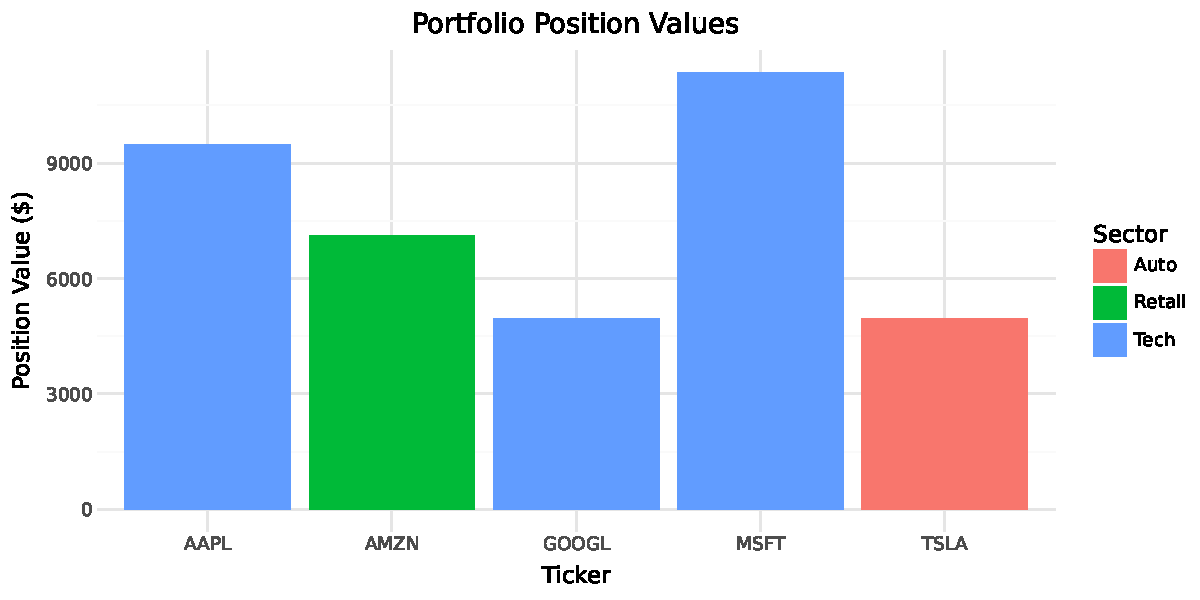
\includegraphics[width=\textwidth]{position_bar.pdf}
\end{column}
\end{columns}

\medskip

Adding \texttt{color="symbol"} in \py{aes()} automatically draws a separate line for each stock.

\end{frame}


\begin{frame}[fragile]{Histogram: Distribution of Returns}

\begin{columns}[T]
\begin{column}{0.48\textwidth}
\begin{lstlisting}[basicstyle=\ttfamily\scriptsize]
aapl = (
    returns_daily
    .filter(
        pl.col("symbol") == "AAPL"
    )
    .to_pandas()
)

(
    ggplot(aapl, aes(x="ret"))
    + geom_histogram(
        bins=50,
        fill="#003366",
        alpha=0.7)
    + labs(
        title="AAPL Daily Returns",
        x="Return", y="Count")
    + theme_minimal()
)
\end{lstlisting}
\end{column}
\begin{column}{0.50\textwidth}
\vspace{1em}
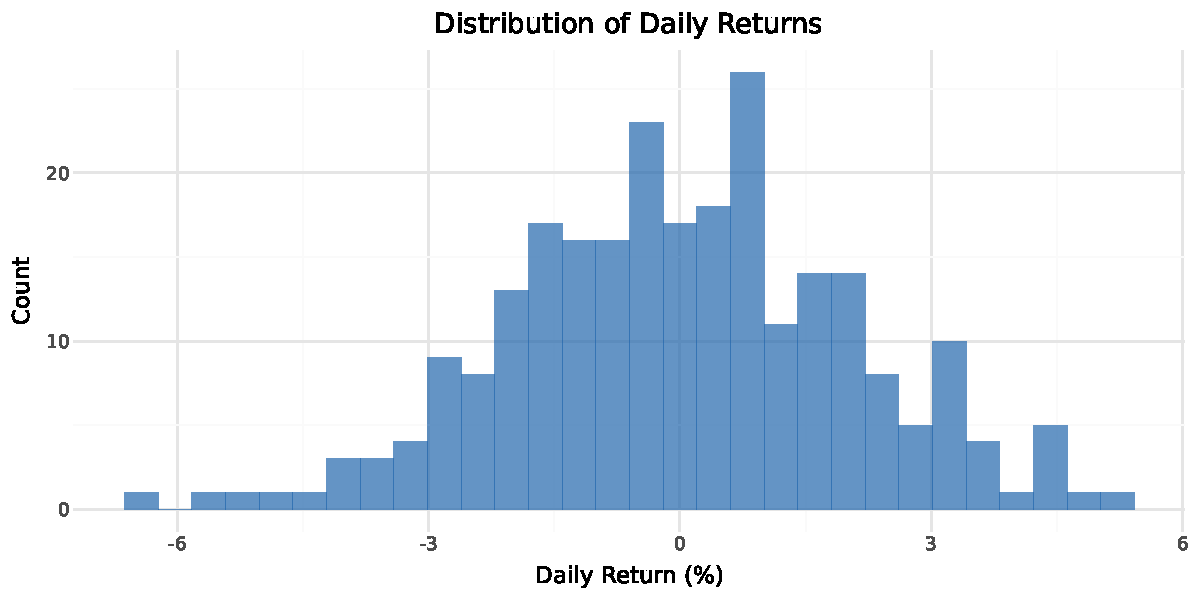
\includegraphics[width=\textwidth]{returns_histogram.pdf}

\smallskip

Returns are roughly bell-shaped but with \textbf{fat tails} --- extreme returns occur more often than a normal distribution predicts.
\end{column}
\end{columns}

\end{frame}


\begin{frame}[fragile]{Cumulative Returns: Growth of \$1}

\begin{columns}[T]
\begin{column}{0.48\textwidth}
\begin{lstlisting}[basicstyle=\ttfamily\scriptsize]
cumulative = (
    returns_daily
    .sort("symbol", "date")
    .with_columns(
        growth=
            (1 + pl.col("ret"))
            .cum_prod()
            .over("symbol")
    )
    .to_pandas()
)

(
    ggplot(cumulative, aes(
        x="date", y="growth",
        color="symbol"))
    + geom_line()
    + labs(title="Growth of $1",
           x="", y="Value ($)")
    + theme_minimal()
)
\end{lstlisting}
\end{column}
\begin{column}{0.50\textwidth}
\vspace{0.5em}
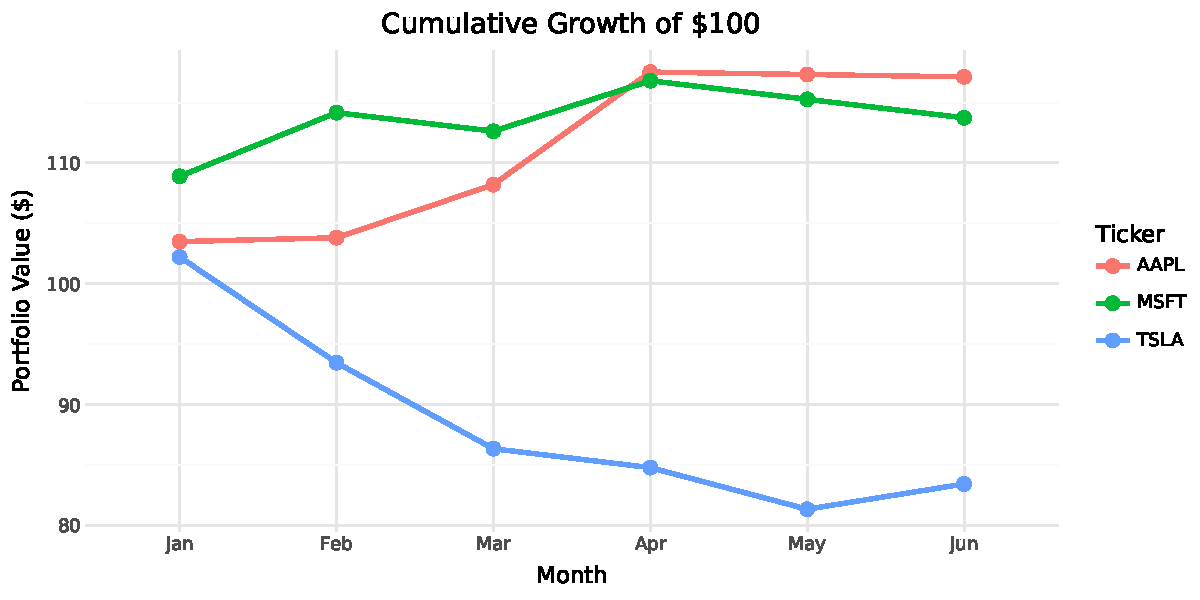
\includegraphics[width=\textwidth]{cumulative_returns.pdf}

\smallskip

\py{.cum_prod()} computes the running product: $(1+r_1)(1+r_2)\cdots(1+r_t)$, showing how \$1 invested on day one grows over time.
\end{column}
\end{columns}

\end{frame}


\begin{frame}{The Key \texttt{geom\_*} Functions}

\begin{tabular}{@{}llp{5.5cm}@{}}
\toprule
\textbf{Geom} & \textbf{Plot type} & \textbf{Use when\ldots} \\
\midrule
\texttt{geom\_col()} & Bar chart & Comparing categories \\[0.4em]
\texttt{geom\_point()} & Scatter plot & Showing relationships between two variables \\[0.4em]
\texttt{geom\_line()} & Line chart & Tracking values over time \\[0.4em]
\texttt{geom\_histogram()} & Histogram & Showing the distribution of a variable \\[0.4em]
\texttt{geom\_smooth()} & Trend line & Adding a fitted line to a scatter plot \\
\bottomrule
\end{tabular}

\bigskip

\begin{highlightbox}
\centering
\textbf{The pattern:} \texttt{ggplot(data, aes(...))} $+$ \texttt{geom\_*()} $+$ \texttt{labs()} $+$ \texttt{theme\_*()}. \\
Swap the \texttt{geom} to change the chart type. Everything else stays the same.
\end{highlightbox}

\end{frame}


\subsection{Exercises}
\begin{frame}[fragile]{Exercise 8: Visualising Data}

\begin{alertblock}{Try It Yourself (5 minutes)}
Using the stock returns data from Exercise 5:
\begin{enumerate}
    \item Plot the adjusted close prices over time for your stocks (use \texttt{geom\_line()})
    \item Create a histogram of daily returns for one stock (use \texttt{geom\_histogram()})
    \item Compute cumulative returns with \py{.cum_prod()} and plot the growth of \$1
    \item \textbf{Bonus:} Map \texttt{color="symbol"} to compare multiple stocks on one chart
\end{enumerate}
\end{alertblock}

\medskip

\begin{highlightbox}
\centering
To save a plot: assign it to a variable and call \texttt{p.save("my\_plot.pdf")}.
\end{highlightbox}

\end{frame}


% ============================================================================
% SECTION 9: SUMMARY
% ============================================================================
\section{Summary}
\subsection{Key Takeaways}

\begin{frame}{What You Learned Today}

\begin{columns}[T]
\begin{column}{0.48\textwidth}
\textbf{Data structures \& I/O}
\begin{itemize}
    \item DataFrames, Series, and data types
    \item \py{read_csv} / \py{write_csv}
    \item \py{read_excel} / \py{write_excel}
    \item \py{scan_csv} for lazy reading
\end{itemize}

\bigskip

\textbf{Expressions \& contexts}
\begin{itemize}
    \item \py{select}, \py{with_columns}, \py{filter}, \py{group_by}
    \item Arithmetic, comparisons, \py{when/then/otherwise}
    \item Casting and expression expansion
\end{itemize}
\end{column}
\begin{column}{0.48\textwidth}
\textbf{Stock returns}
\begin{itemize}
    \item Downloading prices from Yahoo Finance
    \item Computing daily returns with \py{pct_change()}
    \item Window functions with \py{.over("symbol")}
    \item Compounding daily $\to$ monthly returns
\end{itemize}

\bigskip

\textbf{Transformations \& visualisation}
\begin{itemize}
    \item Joins, concatenation, pivot/unpivot
    \item Grammar of Graphics with \texttt{plotnine}
    \item Price charts, return histograms, cumulative growth
\end{itemize}
\end{column}
\end{columns}

\end{frame}


\subsection{Self-Check}
\begin{frame}[fragile]{Quick Self-Check}

\textbf{Can you answer these in your own words?}

\be
    \item What is the difference between \py{read_csv} and \py{scan_csv}?
    \item What is the difference between \py{select} and \py{with_columns}?
    \item Why do we use \texttt{adjusted\_close} instead of \texttt{close} for returns?
    \item What does \py{.pct_change().over("symbol")} do, and why is \py{.over()} needed?
    \item When do you use a \texttt{left} join vs an \texttt{inner} join?
    \item In \texttt{plotnine}, what do \texttt{aes()} and \texttt{geom\_line()} each do?
\ee

\end{frame}


\subsection{Next Steps}
\begin{frame}{What's Next}

\bi
    \item Next week: \alert{panel regression analysis} with financial datasets
    \item \textbf{Homework:} complete today's exercises --- download stock data for your own tickers and explore the returns
    \item Resources:
    \begin{itemize}
        \item Polars user guide: \url{https://docs.pola.rs/}
        \item Polars I/O guide: \url{https://docs.pola.rs/user-guide/io/}
        \item Tidy Finance with Python: \url{https://www.tidy-finance.org/python/}
        \item plotnine gallery: \url{https://plotnine.org/}
    \end{itemize}
\ei

\medskip

\begin{highlightbox}
\centering
If something breaks: read the error message, check your data types, try again.\\
Still stuck? Email me at \href{mailto:ce50@st-andrews.ac.uk}{ce50@st-andrews.ac.uk}.
\end{highlightbox}

\end{frame}


\end{document}
